\chapter{ Ambiente di Lavoro}

\section{Windows e TeXnicCenter}

Durante la prefazione (che nessuno di voi avr\`a certamente letto) abbiamo
parlato di IDE. Per il nostro corso ne utilizzeremo uno, molto semplice da
usare ma anche molto pratico. Si chiama \textit{TeXnicCenter}, e in questo
capitolo vedremo un attimo le sue funzionalit\`a, giusto per prendere mano
con l'ambiente che dovremo usare.

Prima di tutto, alla apertura del programma ci troveremo ad una schermata
vuota, in cui possiamo vedere diversi bottoni.

\begin{figure}[H]
  \centering
  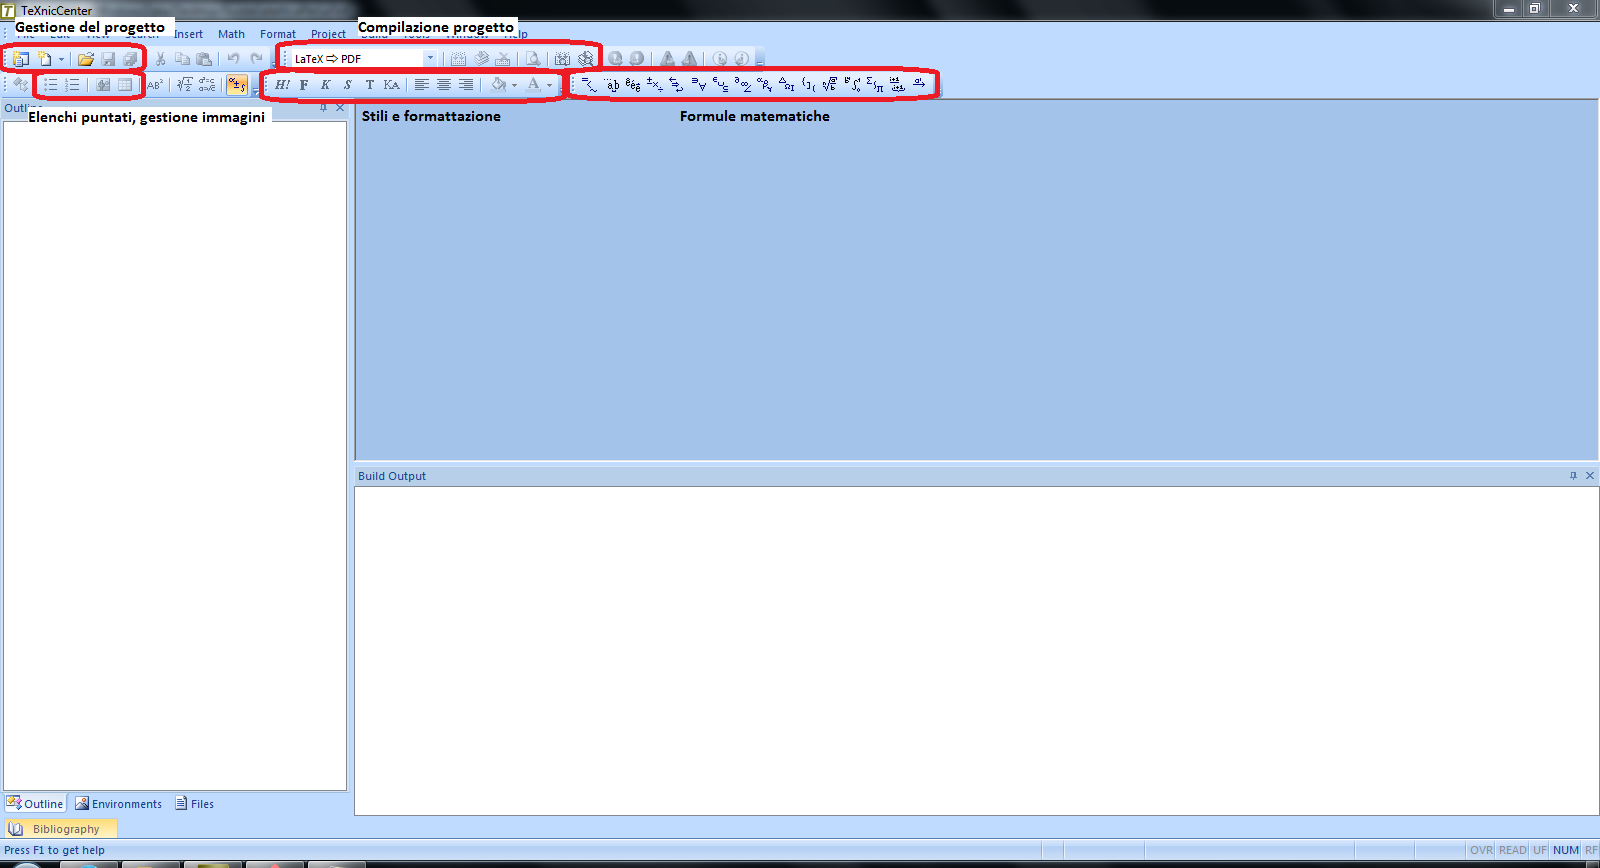
\includegraphics[scale=0.35]{texniccenterprincipale}
  \caption{Schermata principale di TeXnicCenter}
\end{figure}

Come possiamo vedere dall'immagine\footnote{Sappiamo che si vede poco
ma questo \`e il meglio che siamo riusciti a fare} notiamo partendo da in alto
a sinistra e scorrendo verso destra che inizialmente troviamo dei bottoni per
gestire il progetto (o per crearne di nuovi).
Abbiamo subito dopo le opzioni per la compilazione: il men\`u a tendina ci
permette di selezionare che tipo di output vogliamo (se PDF o altri formati) e
i bottoni accanto a questo men\`u ci permettono di lanciare la compilazione
del progetto.
Nella seconda riga troviamo le impostazioni per aggiungere elenchi puntati e
numerati, seguiti dai bottoni per aggiungere immagini e tabelle. Nel penultimo
riquadro ci sono i classici bottoni per impostare gli stili di formattazione
(quelli che siamo abituati ad avere in Word per intenderci).
Alla fine troviamo i bottoni per l'inserimento di formule matematiche, che
tratteremo pi\`u avanti in questa guida.

\subsection{Creare un progetto}

Iniziamo ora la creazione di un progetto.
Clicchiamo su \texttt{New Project} e selezioniamo l'unico modello diponibile,
ovvero quello vuoto. Spuntiamo la casellina \texttt{Uses BibTeX} nella sezione
\texttt{Features}, e diamo un nome al nostro progetto. Fatto ci\`o il bottone
\texttt{Ok} dovrebbe essersi sbloccato, e lo clicchiamo. Il programma creer\`a
le basi necessarie per cominciare un nuovo progetto!\footnote{Nota, se volete
potete selezionarvi il percorso dove salvare il progetto che preferite.}